\documentclass[11pt,oneside,a4paper,notitlepage]{article}

\usepackage[utf8]{inputenc}
\usepackage[ngerman]{babel}
\usepackage[margin=1.5cm]{geometry}

%kommentare, zitate, quellcode
\usepackage{verbatim}
%\fontfamily{sfdefault}
\renewcommand{\familydefault}{\sfdefault}
%
\usepackage{graphicx}
%fuer tabellen
\usepackage{tabularx}
\usepackage{tabulary}
%
%formatierung listen
\let\oldenumerate\enumerate
\renewcommand{\enumerate}{
  \oldenumerate
  \setlength{\itemsep}{1pt}
  \setlength{\parskip}{0pt}
  \setlength{\parsep}{0pt}
}

%
%referenzen und links
\usepackage{hyperref}
\hypersetup{
colorlinks=true,
linkcolor=cyan,
urlcolor=cyan,
hidelinks=false
}
%
% 
\renewcommand{\arraystretch}{1.5}
%

\begin{document}
%
\section{System \& Nutzerinformationen}

Zur Vorbereitung der Anforderungsanalyse werden hier einige Informationen zum System und deren Benutzer zusammengetragen.


\section{Systemprozess}
%
Ausgehend von \href{EISWS1516Howe_Domaenenrecherche.pdf}{Domänenrecherche (Prozess)} die Darstellung eines exemplarischen Verarbeitungsprozesses\\

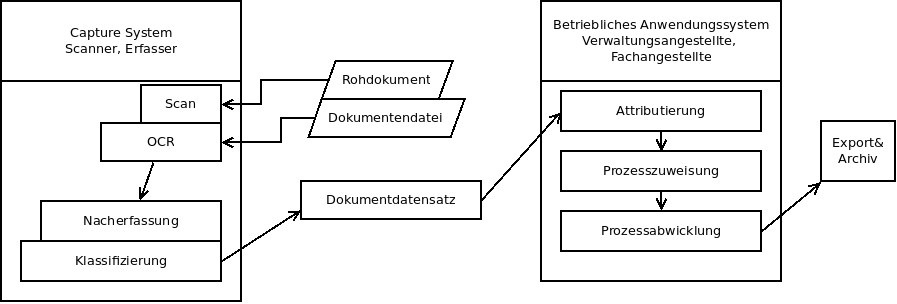
\includegraphics[width=\textwidth]{EISWS1516Howe_Prozess_deskriptiv.png}
\noindent




%
\end{document}

